\documentclass[Unicode]{article}
\usepackage{graphicx}
\usepackage{geometry}
\usepackage{amsmath}
\usepackage{listings}
\geometry{a4paper,scale=0.6}

\title{A Solution Manual for Introduction to Algorithms}
\author{Jiawen Bi}

\begin{document}

\maketitle
\tableofcontents

\section{Foundations}

\section{Getting Started}
\subsection{Insertion sort}
\textbf{\textit{\Large{2.1-1}}}\\
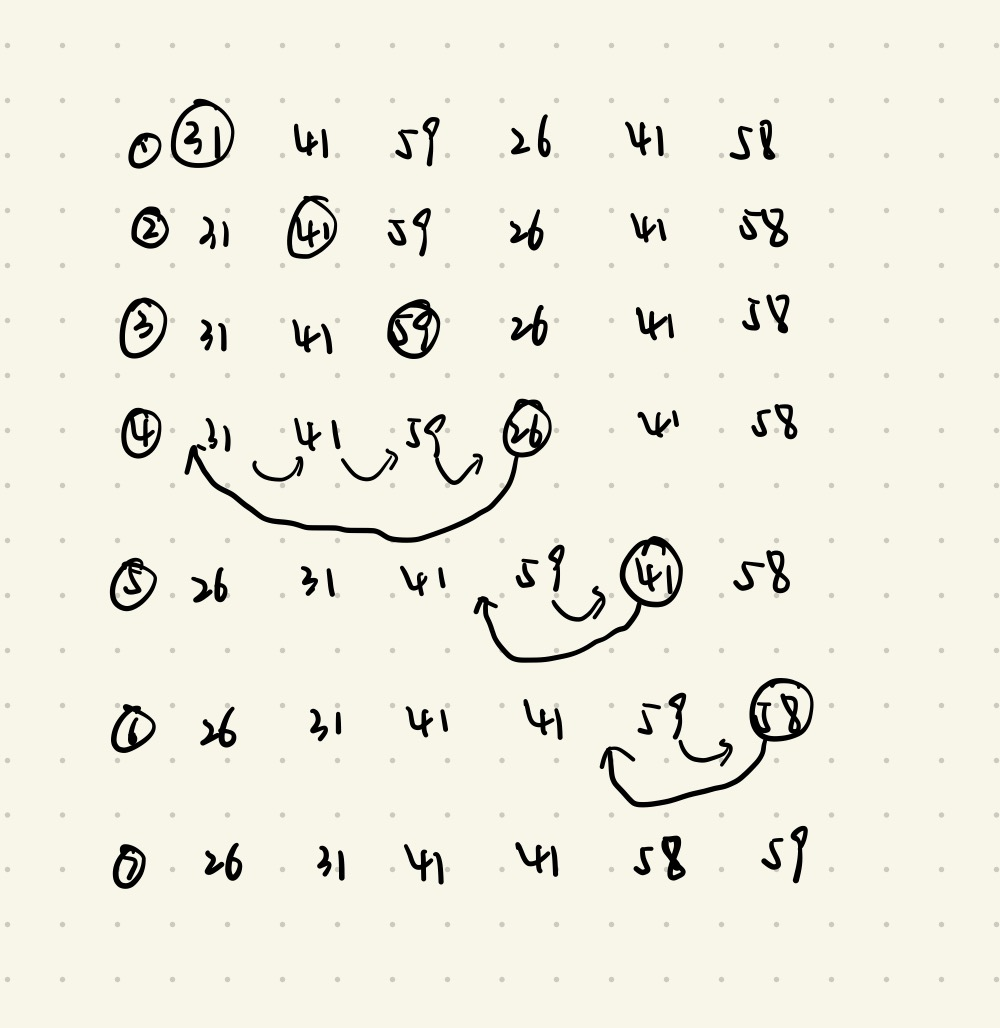
\includegraphics[scale=0.2]{c.jpeg}\\
\textbf{\textit{\Large{2.1-2}}}
\begin{lstlisting}[language=Python,numbers=left,numberstyle=\normalsize]
for j = 2 to A.length
    key = A[j]
    i = j -1 
    while i > 0 and A[i] < key
        A[i + 1] = A[i]
        i = i - 1
    A[i+1] = key
\end{lstlisting}
\textbf{\textit{\Large{2.1-3}}}
\begin{lstlisting}[language=Python,numbers=left,numberstyle=\normalsize]
#linear search
for i = 1 to A.length
    if v = A[i]:
        return i
return NIL
\end{lstlisting}
\textbf{\textit{\Large{2.1-4}}}\\
\textbf{Input} : two integer arrays A and B such that $A.length=B.length=n$, and
$ \forall i \in \{0,2,\cdots,n-1\}, A[i],B[i] \in \{0,1\} $\\
\textbf{Output} : a integer array C such that $C.length=n+1$, and
$ \forall i \in \{0,\cdots,n\}, C[i]\in \{0,1\} $, and $c=a+b$, where a,b,c represents the decimal integers of A,B,C
\begin{lstlisting}[language=Python,numbers=left,numberstyle=\normalsize]
for i = n-1 to 0
    C[i] = (C[i+1] + A[i] + B[i]) / 2
    C[i+1] = (C[i+1] + A[i] + B[i]) % 2
return C
\end{lstlisting}

\end{document}